\testsection{Library: Units in labels}
\usepgfplotslibrary{units}

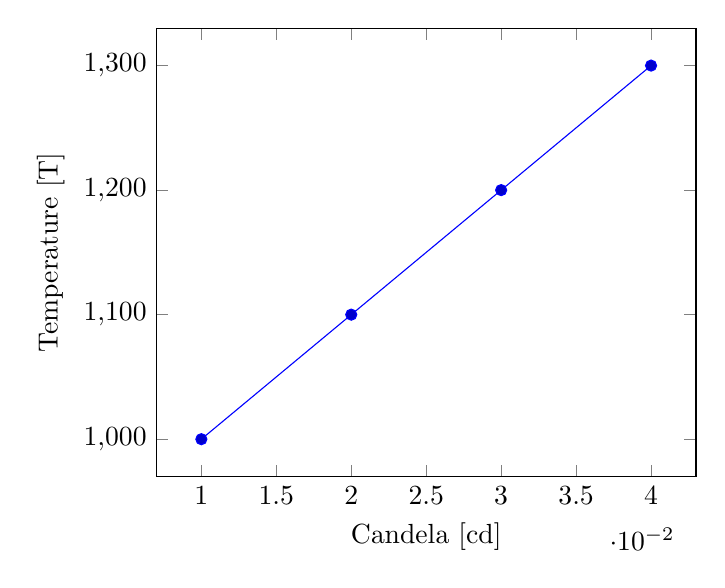
\begin{tikzpicture}
  \begin{axis}[xlabel=test,x unit=cd,xlabel=Candela,y unit=T,ylabel=Temperature]
    \addplot coordinates {
        (0.01,1000)
        (0.02,1100)
        (0.03,1200)
        (0.04,1300)
    };
  \end{axis}
\end{tikzpicture}

With scaled

\begin{tikzpicture}
  \begin{axis}[change y base,y SI prefix=kilo,change x base,x SI prefix=centi,x unit=T,unit code/.code 2 args={\mathbf{#1}\mathrm{#2}},ylabel=Test]
    \addplot coordinates {
        (0.01,1000)
        (0.02,1100)
        (0.03,1200)
        (0.04,1300)
    };
  \end{axis}
\end{tikzpicture}

With prefix no scale

\begin{tikzpicture}
  \begin{axis}[y SI prefix=kilo,x SI prefix=micro,x unit=T,xlabel=test]
    \addplot coordinates {
        (0.01,1000)
        (0.02,1100)
        (0.03,1200)
        (0.04,1300)
    };
  \end{axis}
\end{tikzpicture}



%%% Local Variables: 
%%% mode: latex
%%% TeX-master: "pgfplotstest"
%%% End: 
